\documentclass[12pt,onecolumn,letterpaper]{article}

%\usepackage{cvpr}
\usepackage{times}
\usepackage{epsfig}
\usepackage{graphicx}
\usepackage{amsmath}
\usepackage{amssymb}
\usepackage{listings}
\lstloadlanguages{Python}
\lstset{language=Python,tabsize=2,basicstyle=\tiny}
\usepackage[margin=1in]{geometry}
\usepackage{float}
\usepackage{caption}
\usepackage{subcaption}
\captionsetup{compatibility=false}

\usepackage{subcaption}

\usepackage{multirow}

\usepackage{graphics}
\graphicspath{{images/}}
\usepackage{url} 


% Include other packages here, before hyperref.

% If you comment hyperref and then uncomment it, you should delete
% egpaper.aux before re-running latex.  (Or just hit 'q' on the first latex
% run, let it finish, and you should be clear).
\usepackage[breaklinks=true,bookmarks=false]{hyperref}

%\cvprfinalcopy % *** Uncomment this line for the final submission

\def\cvprPaperID{****} % *** Enter the CVPR Paper ID here
\def\httilde{\mbox{\tt\raisebox{-.5ex}{\symbol{126}}}}

% Pages are numbered in submission mode, and unnumbered in camera-ready
%\ifcvprfinal\pagestyle{empty}\fi
\setcounter{page}{1}
\begin{document}

%%%%%%%%% TITLE
\title{STAT361 Final Report: Classification of Unknown Substances Using Support Vector Machine}

\author{Yutaro Yamada\\
Yale University\\
{\tt\small yutaro.yamada@yale.edu}
}


\maketitle
%\thispagestyle{empty}

%%%%%%%%% ABSTRACT
\begin{abstract}

This paper investigates a spectra dataset in order to build a classification model that determines if a substance is benign or causative agent for anthrax, which is an acute dangerous disease. To reduce the noise of the sample data, outliers are excluded based on the plots of the dataset. Feature extraction is done via two different methods. The first approach employs Principle Component Analysis, and the number of principle components to include in a reduced matrix is determined by the scree plot. The second method utilizes linear regression, which effectively reduces the size of features. Both models are trained via Support Vector Machine. The model based on the first method produces unstable classification results on a test set when the number of principle components is small. The model based on the second method is more reliable since it produces 100\% accuracy on all the validation sets. The first model with 6 principle components and the second model agree with the prediction such that the fifth and ninth substance on the test set are classified as anthrax. The comparison of two methods shows that the prior knowledge of a certain substance helps improving classification accuracy. Other methods that incorporate external information other than sample dataset could be further studied for better classification accuracy. 

\end{abstract}



%%%%%%%%% BODY TEXT
\section{Introduction}

Anthrax is the harmful disease caused by the bacteria \textit{Bacillus anthracis}. Due to its high lethality and durability, when an area has been contaminated by substances that could potentially contain anthrax, there needs to be an efficient and quick way to detect if a substance is benign or anthrax. Laser-induced breakdown spectroscopy (LIBS) is one of the methods which aid in determining the existence of anthrax based on characteristic spectra generated by LIBS devices. Although spectra data with wavelengths for different substances can be easily obtained by LIBS, it is difficult to distinguish if a substance is anthrax or not due to high variability of the spectra data. In such a classification task, dimensionality reduction is often employed to extract important features that are effective in classification. Such reduction of complexity not only improves classification accuracy due to its noise reduction effect, but also helps building a model that is generalized well. In this paper, two dimensionality reduction methods are explored: singular value decomposition and linear regression approach in an attempt to obtain highly generalized predictability to correctly classify unknown substances.        
 
\section{Method}

% Brief overall summary of methods that I used. I should write after I finish everything.
We first performed exploratory data analysis and attempted to detect outliers. We then prepared training data as a set of data samples and class labels. We applied principle component analysis and linear regression to extract useful features. We performed SVM for building a classification model, and tested its performance on the provided test dataset.   

\subsection{Exploratory data analysis}

As we plotted the spectra of various substances, we observed that some of the examples do not follow the pattern similar to the majority of other points. We created a plotting function and visually compared each plot in the same group of substances in order to detect outliers. Although the initial attempt was to exclude as many outliers as possible, it turned out that many of the substances have high variability among the same group, resulting in excluding only one sample as an outlier. The sample that we excluded is shown in the Figure 1 along with its corresponding median spectrum of the others in the same group.   

\begin{figure}[htbp]
  \centering
    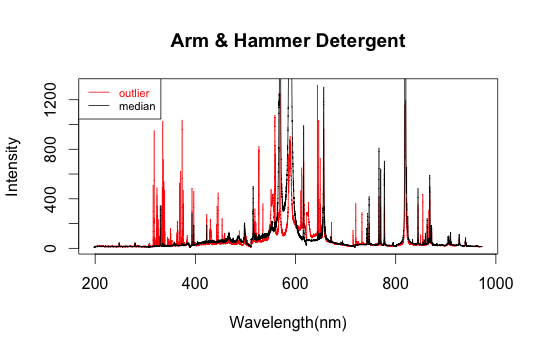
\includegraphics[width=.8\linewidth]{armh_fin}
    \caption{The outlier example in armh.txt}
  \label{fig:1}
\end{figure}
 
\subsection{Training data preparation}

After the initial EDA, we combined all the data available to us to create a training matrix X. The data samples used are: anthrax1, anthrax2, anthrax3, Arm \and Hammer Detergent, Rumford Baking Powder, Arm and Hammer Baking Soda, Crayola Chalk, Food Lion Brand flour, Advil Ibuprofen tablets, Food Lion Brand Sugar, Tide Laundry Detergent, and Tylenol Acetaminophen Capsules. We also created a y vector to store classification labels \{1, 2\}, where "1" stands for anthrax and "2" stands for substances that are not anthrax. We performed random permutation of data samples.

We then normalized the matrix X so that it has zero mean for each column. This centering ensures that the first principle component indeed is the direction of the maximum variability of the original data cloud since we do not need to think about the intercept after centering. We did not perform column scaling in favor of preserving the variability among features because it could contain meaningful information.  

\subsection{Dimensionality Reduction}

What we wanted was to extract useful features that capture characteristic peaks and shapes of the spectra data so that we can train a model based on those features to distinguish anthrax from other substances.  

We applied two types of dimensionality reduction. The first approach employs principle component analysis and the second approach utilizes linear regression based on a prior knowledge of chemical compounds that anthrax consists of.  

\subsubsection{Method 1: Principle Component Analysis}

We applied Singular Value Decomposition on the training data matrix X, obtaining U, $\Sigma$, and V. We created a truncated X by multiplying the first k columns of U with the first k columns of $\Sigma$, where k is determined by the scree plot. Since T = XV = U$\Sigma$, this is equivalent to linearly re-parameterize the matrix X such that each new coordinate in T is uncorrelated with the others, and the first component has the largest variance of all linear combinations of the columns of X. We used the V matrix as a loading matrix to translate the test data to the same coordinate system as the truncated training data. 

We plotted the singular values in $\Sigma$ to decide how many of principle components to use to create a reduced matrix X (Figure 2 (a)). 

We also tried different values for k and compared the testing accuracy on validation sets. When we calculated the accuracy, we subsetted the training data into 10 groups, used one of them as a validation set, and repeated this procedure to take the average accuracy (Figure 2 (b)).


\begin{figure}[thbp]
  \centering
  \begin{subfigure}{.4\textwidth}
  \centering
    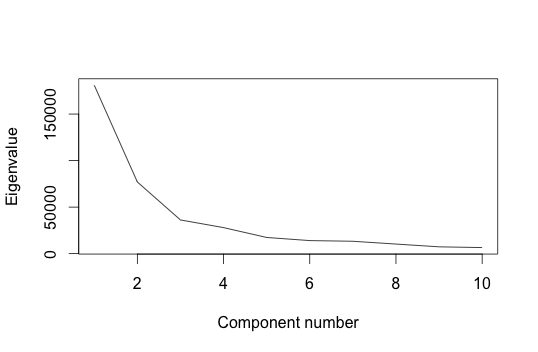
\includegraphics[width=\linewidth]{scree}
    \caption{The scree plot for the first 10 principle components}
    \label{fig:sub1}
  \end{subfigure}
  \begin{subfigure}{.4\textwidth}
    \centering
    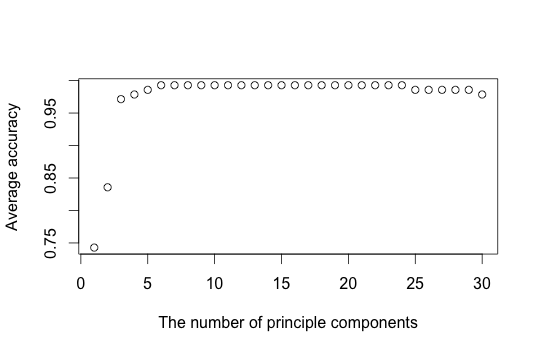
\includegraphics[width=\linewidth]{acc_pc}
    \caption{The average accuracy v. the number of principle component}
    \label{fig:sub2}
  \end{subfigure}
  \caption{}
  \label{fig:2}
\end{figure}

We see that when the number of principle components is larger than 25, the average accuracy starts to decrease. This might stem from the fact that it incorporates too much noise in the model, making it less accuracy. Based on these two plots, we chose k = 6 for our model.  

\subsubsection{Method 2: Linear Regression}

Given the information that anthrax consists of B$_{2}$O$_{3}$, graphite, CaClO${_3}$, FeSO${_4}$, KI, MgSO${_4}$, MnSO$_4$, NaCl, and Si, we applied linear regression to obtain estimated coefficients of these chemical compounds for anthrax. We took the median of each chemical substance and used them in the model. We took each row of X as a dependent variable and a set of chemical substances as independent variables, and we performed multivariate linear regression on them. 

As a result, we obtained a reduced matrix, where each row corresponds to a chemical substance that we included in the linear model, and each column corresponds to a data sample. This method is indeed another way of representing the original matrix in the low dimensional space because 13701 features are now reduced to 9 features; we can think that each feature in the original space is projected onto the 9 dimensional spaces, where the hyperplane that separates Anthrax from other substances can be more easily calculated. 

\subsection{Training using Support Vector Machine}

We chose Support Vector Machine as our classification method. We used "e1071" R package to perform binary SVM, which is a method that determines a hyperplane that separates the high dimensional data space into two classes, which represent \textit{Anthrax} or \textit{Benign}. 


\subsection{Testing}

In order to apply our model to the test case, we first centered the test case. For PCA, we multiplied the V matrix from the training set to create a truncated test data matrix X. For linear regression, we performed the same linear regression on the entire test X to get the reduced matrix. We then provide the test matrix to the prediction function of SVM and obtained our prediction. 


\section{Results}

\subsection{Validation result}

In order to measure the performance of our model using the training set, we performed the 10-fold cross validation.

\subsubsection{Method 1: PCA}

As chosen in the method section, we performed the cross validation with k = 6, where k is the number of principle components. Since we subsetted the training set into 10 groups, we performed 10 times of training and validation. The average training accuracy was 100\%. The average validation accuracy was 99.26\%. 

\subsubsection{Method 2: Linear Regression}

Similarity, we performed the cross validation on the second model, and the average accuracy was 100\% for both training and validation.

The SVM model learns the combination of coefficients of chemical compounds that make up anthrax. This makes the classification task easier and more accurate than the method 1 because the data points for anthrax will be concentrated into one place, which means that determining the hyperplane that distinguishes anthrax from other substances in this space is easier than the previous method where it needs to determine potentially highly non-linear hyperplane.  

\subsection{Test result}

Both models predict the 5th and 9th substance as Anthrax. The whole result is shown in table 1.  

\begin{table}[hbtp]
  \caption{Predicted Classes} 
  \label{table:prediction}
  \centering
  \begin{tabular}{ccc}
    \hline
    Test case substance  &       &  Classification  \\
    \hline \hline
    1  &   &  Benign \\
    2  &    & Benign \\
    3  &   &  Benign \\
    4  &    &  Benign \\
    5  &    &  Anthrax \\
    6  &    &  Benign \\
    7  &    &  Benign \\
    8  &    &  Benign \\
    9  &    &  Anthrax \\
    10  &    &  Benign \\
    \hline
  \end{tabular}
\end{table}



\section{Discussion}

We investigated a spectra dataset and built a binary classification model in order to determine if a substance is Anthrax or not. We tested two different methods of dimensionality reduction. Both models agreed on their prediction on the test dataset.  

Possible shortcomings of the analysis is that our model might not be generalized enough to provide accurate prediction for unknown substances due to the relatively small number of data samples. More data samples could contribute to building a more accurate model. 

We observed that the model 2 was better than the model 1 in terms of accuracy on the validation sets. One reason that explains the difference in predictability is that the model 2 utilizes the information of chemical compounds that anthrax consists of, which greatly helps revealing the internal structure of high dimensional data cloud, aiding the better classification result. 

This observation suggests two useful insights: 1. researchers could effectively employ external information other than the provided data in order to better understand the provided data, which helps obtaining better accuracy of a model. The second insight is that there might be other external information that potentially helps understanding the data more.   

\subsection{Similarity between speech recognition task}

Initially, we tried to incorporate some insights from our observation that log-transformed spectral data from laser-induced breakdown spectroscopy are similar to the Fourier-transformed sound wave data often used in speech recognition tasks.

We read the paper \cite{cisewski} cited in the final report description sheet for our reference, and noticed that they had used logarithmic data transformation. When we applied logarithmic transformation to some of the provided sample data, we noticed the geometrical similarity between our spectral data and sound wave data often used in speech recognition.  

However, further research revealed that MFCC feature extraction methods were specifically designed to capture particular characteristics of human voices for speech recognition. Therefore, we stopped further exploration in this direction.

Although we did not apply MFCC feature extraction in our approach, as the method 2 suggests, other feature extraction methods which incorporate domain specific knowledge could be further studied for better classification accuracy. 


{\small
\bibliographystyle{ieee}
\bibliography{egbib}
}

\begin{thebibliography}{1}

  \bibitem{cisewski} Cisewski, J., Snyder, E., Hanning, J. and Oudejans, L. (2012), {\em Support vector machine classification of suspect powders using laser-induced breakdown spectroscopy (LIBS) spectral data} : J. Chemometrics, 26: 143-149


\end{thebibliography}




{\small
\bibliographystyle{ieee}
\bibliography{egbib}
}

\end{document}
